% Apresentação de resultados da PoC OCR-06 (INE5448, 17/11/2026), 5 minutos
\documentclass[aspectratio=169,11pt]{beamer}
\usetheme{metropolis}
\usepackage[utf8]{inputenc}
\usepackage[T1]{fontenc}
\usepackage[brazil]{babel}
\usepackage{booktabs}
\usepackage{xcolor}
\usepackage{array}
\metroset{progressbar=frametitle, numbering=fraction}
\setbeamertemplate{caption}{\insertcaption}
\definecolor{bom}{HTML}{1B8A62}
\definecolor{ruim}{HTML}{C0392B}
\newcommand{\ok}[1]{\textcolor{bom}{#1}}
\newcommand{\erro}[1]{\textcolor{ruim}{#1}}

\title{OCR-06: OCR Adaptativo com Aprendizagem Assistida}
\subtitle{Resultados da PoC}
\author{Gabriel Salmoria \quad {\small Tutor: Lucas Mayr}}
\institute{INE5448 -- IA e Segurança -- UFSC}
\date{17 de novembro de 2026}

\begin{document}

\maketitle

% ------------------------------------------------------------------ 1. onde paramos
\begin{frame}{O plano da apresentação intermediária}
\textbf{Proposta:} LoRA no Chandra OCR 2 com \textbf{linhas} manuscritas
\begin{itemize}
  \item Caligrafia real do BRESSAY (redações) e linhas sintéticas com nomes do IBGE, TSE e Receita
  \item Nomes só como contagens agregadas, nenhuma linha corresponde a uma pessoa
\end{itemize}
\vspace{0.6em}
\textbf{Em linhas, funcionou} (quarta entrega)
\begin{itemize}
  \item CER no BRESSAY: 20,1\% $\rightarrow$ 4,9\%
  \item Nomes nunca vistos lidos sem erro: 70,9\% $\rightarrow$ 79,7\%
  \item Sem sinal de memorização (diferença vistos/inéditos: 2,3 $\rightarrow$ 2,1 pontos de CER)
\end{itemize}
\end{frame}

% ------------------------------------------------------------------ 2. por que não bastou
\begin{frame}{Por que não bastou: o Chandra lê páginas, não linhas}
\small
O mesmo adaptador de linhas aplicado em páginas inteiras:
\vspace{0.4em}

\centering
\begin{tabular}{@{}lrr@{}}
\toprule
Campos manuscritos exatos, página inteira & Chandra & Ajustado em linhas \\
\midrule
Certidões do OCRSD (47 págs.) & 84,7\% & 84,4\% \\
Certidões geradas (38 págs.) & 56,6\% & 55,4\% \\
\quad só nomes & 19,9\% & 22,7\% \\
\bottomrule
\end{tabular}

\vspace{0.6em}
\raggedright
\begin{itemize}
  \item O uso real é a página inteira, e o adaptador só tinha visto recortes de uma linha
  \item O ganho das linhas quase não chegou aos campos de uma certidão
  \item Decisão: treinar com \textbf{páginas inteiras}, no formato HTML nativo do Chandra
\end{itemize}
\end{frame}

% ------------------------------------------------------------------ 3. nova abordagem
\begin{frame}{Nova abordagem: páginas inteiras de Registro Civil}
\begin{itemize}
  \item \textbf{Alvo}: o HTML de layout do Chandra, com o texto impresso copiado da saída dele
  \item \textbf{Dados}: 1.000 páginas do gerador OCRSD (ONR) e 2.500 geradas localmente, em 5 modelos (certidões de nascimento, casamento e óbito, DNV)
  \item \textbf{Perda ponderada}: impresso 0,3, manuscrito 1; no lora\_v2, nomes com peso 2 e peso extra quando o modelo erra
  \item \textbf{Duas etapas}: lora\_v1 (1.800 págs., a partir do Chandra) e lora\_v2 (+1.700 págs.), cerca de 65 min cada na RTX PRO 6000
  \item \textbf{Teste}: 200 páginas fora do treino, 100 \emph{difíceis} (70\% das palavras de nome nunca vistas) e 100 \emph{normais} (nomes pela frequência real)
\end{itemize}
\end{frame}

% ------------------------------------------------------------------ 4. gerador
\begin{frame}{Como as páginas locais são geradas}
\begin{columns}[T]
\begin{column}{0.33\textwidth}
\centering
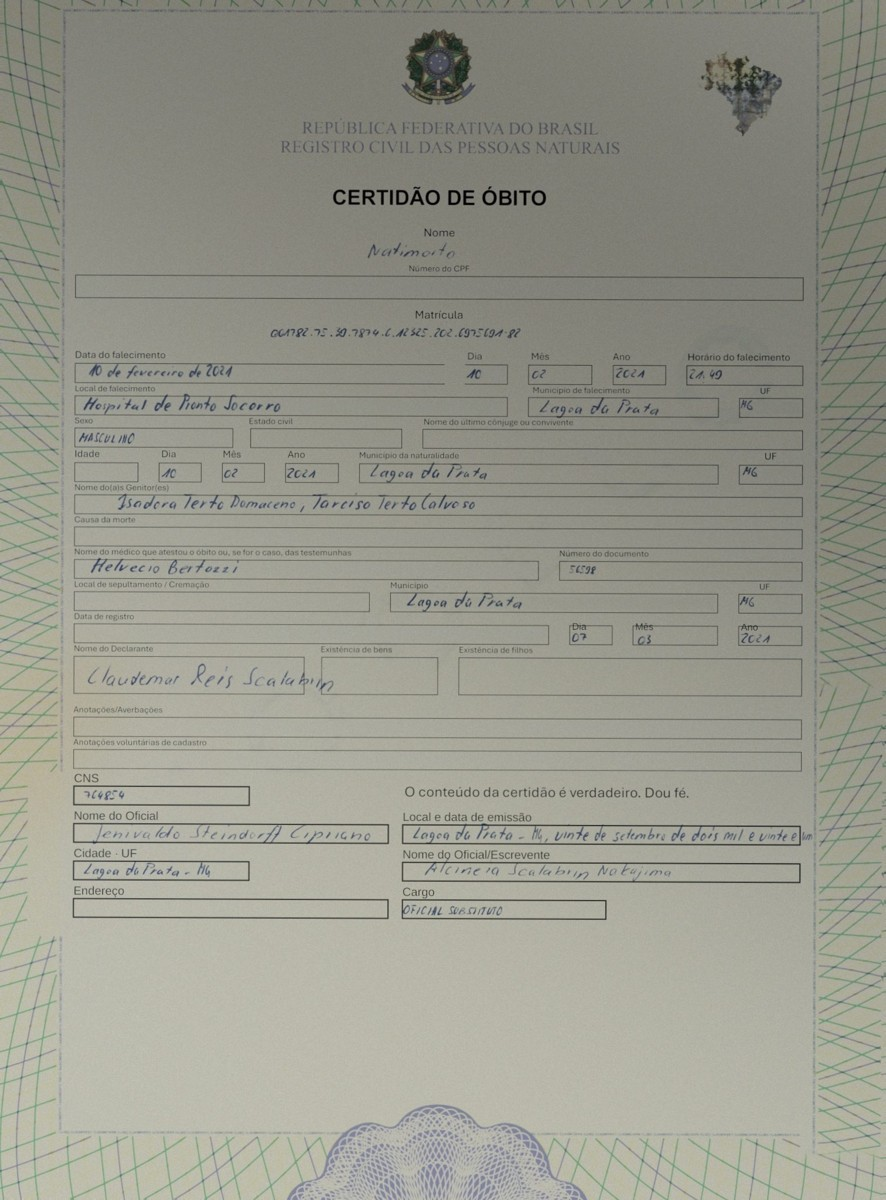
\includegraphics[height=0.76\textheight]{figs/gerador_pagina.jpg}

\scriptsize Certidão de óbito do teste difícil, VATr++, nível 2
\end{column}
\begin{column}{0.64\textwidth}
\small
\begin{itemize}
  \item \textbf{Modelo}: modelos em branco e mapas de campos do OCRSD, em 5 documentos de Registro Civil: casamento (antiga e CNJ), nascimento (CNJ), óbito e DNV
  \item \textbf{Registro}: um registro do OCRSD re-sorteado; cada prenome, sobrenome e município troca na página inteira por um do léxico (IBGE, TSE, Receita), respeitando a partição treino/teste
  \item \textbf{Mão}: uma mão e uma caneta por página, com 85 fontes ou os geradores neurais VATr++ e Graves (estes só escrevem texto sem acento)
  \item \textbf{Dificuldade}: níveis 1 a 4, com letras deformadas e fundidas, falhas e borrões, papel com sombra, ruído e JPEG
\end{itemize}
\end{column}
\end{columns}
\end{frame}

% ------------------------------------------------------------------ 4b. detalhe
\begin{frame}{Página gerada, em detalhe}
\centering
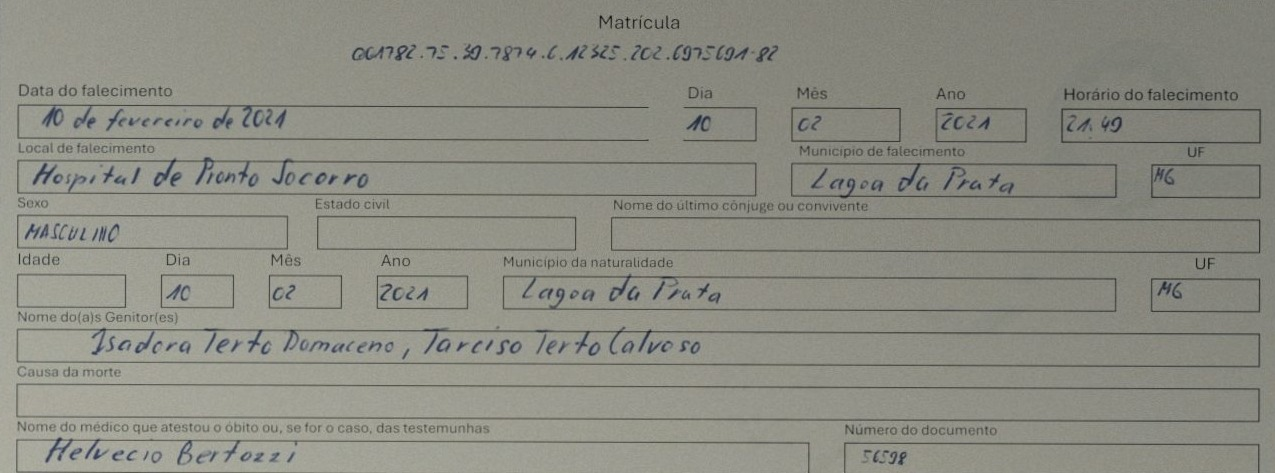
\includegraphics[width=0.80\textwidth]{figs/gerador_zoom_1.jpg}

\vspace{0.4em}
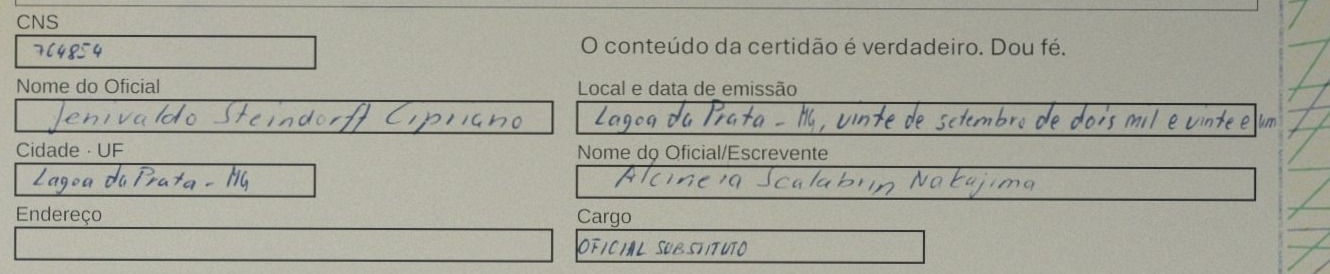
\includegraphics[width=0.80\textwidth]{figs/gerador_zoom_2.jpg}
\end{frame}

% ------------------------------------------------------------------ 5. resultados
\begin{frame}{Resultados por tipo de campo}
\centering
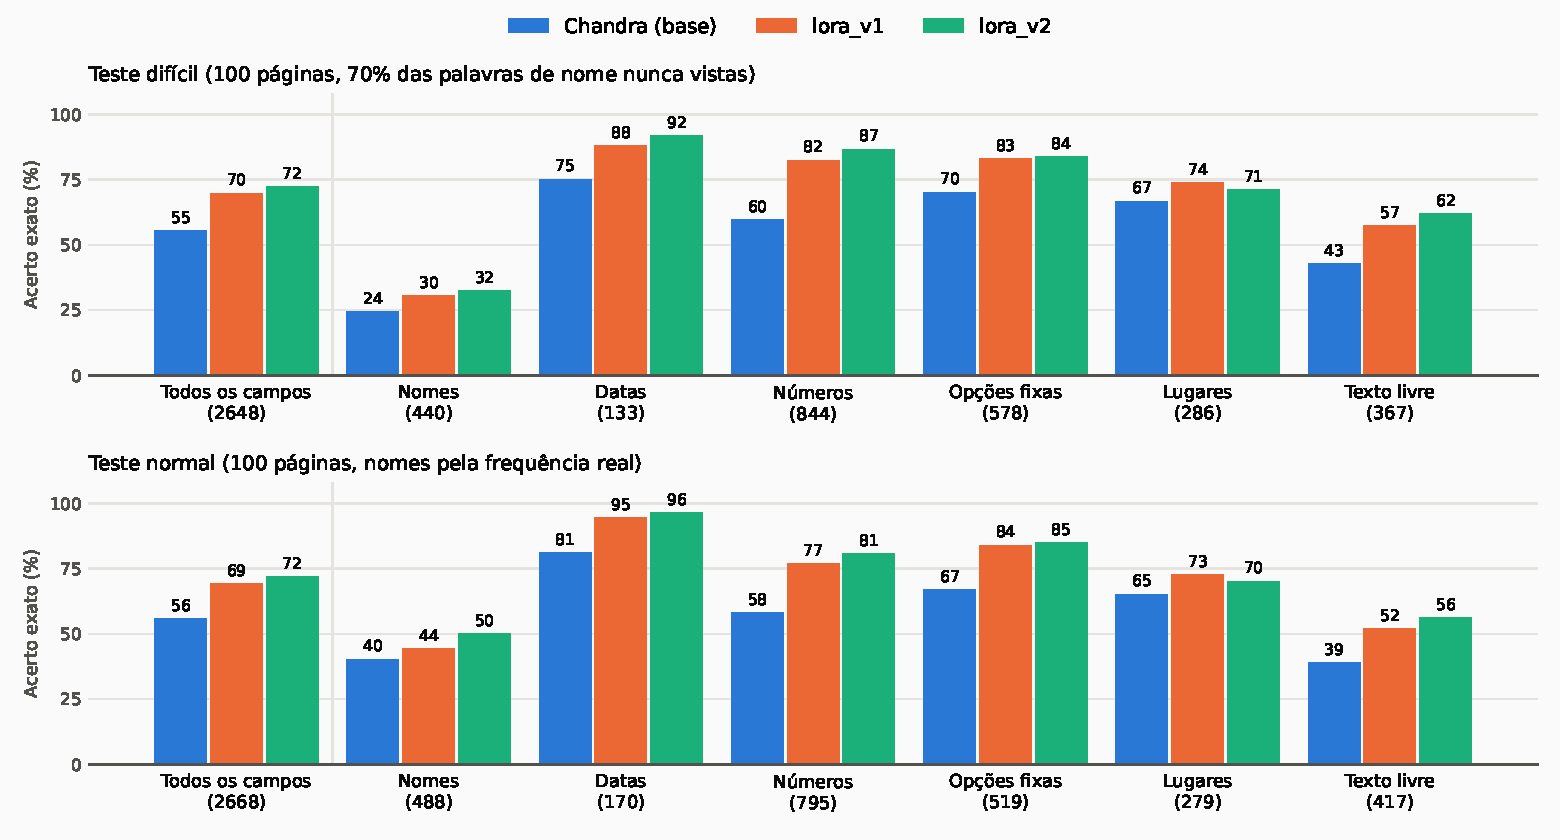
\includegraphics[width=0.82\textwidth]{figs/resultados.pdf}

\vspace{-0.2em}
\scriptsize
lora\_v2 sobre o Chandra (difícil / normal): \textbf{+16,8 / +16,2} pontos nos campos, \textbf{+8,2 / +9,8} nos nomes; IC 95\% $>$ 0
\end{frame}

% ------------------------------------------------------------------ 5. exemplos
\begin{frame}{Como ficam os erros de nome}
\footnotesize
\centering
\renewcommand{\arraystretch}{1.15}
\begin{tabular}{@{}m{4.0cm}m{3.3cm}m{3.4cm}m{2.0cm}@{}}
\toprule
Imagem & Gabarito & Chandra & lora\_v2 \\
\midrule
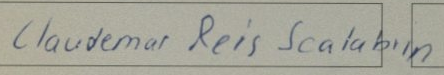
\includegraphics[width=3.8cm]{figs/nome_1.png} & Claudemar Reis Scalabrin & Claude\erro{mi}r Reis Scalabrin & \ok{igual} \\
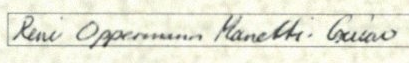
\includegraphics[width=3.8cm]{figs/nome_2.png} & Reni Oppermann Manetti Guiao & \dots{} Manett\erro{e} \erro{Greco} & \ok{igual} \\
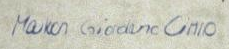
\includegraphics[width=2.8cm]{figs/nome_3.png} & Maikon Giordano Cirino & \erro{Manoel} Giordan\erro{e} \erro{Critto} & \erro{Marcia} \dots \\

\includegraphics[width=3.6cm]{figs/nome_4.png} & Guiomar Schiavon Arrabal & \erro{Geovana} Schiav\erro{e}n \dots & \erro{Giovana} \dots \\
\bottomrule
\end{tabular}

\vspace{0.5em}
\raggedright
O erro que sobra é o da proposta original: o prenome raro vira um prenome comum
\end{frame}

% ------------------------------------------------------------------ 6. quantização
\begin{frame}{Comparação dos modelos}
\scriptsize
\centering
\renewcommand{\arraystretch}{1.0}
\setlength{\tabcolsep}{5pt}
\begin{tabular}{@{}lcc|c|ccc@{}}
\toprule
 & \multicolumn{2}{c|}{\textbf{Chandra OCR 2}} & \textbf{lora\_v1} & \multicolumn{3}{c}{\textbf{lora\_v2}} \\
 & BF16 & FP8 & BF16 & BF16 & FP8 & INT4 \\
\midrule
\multicolumn{7}{@{}l}{\textit{Teste difícil (100 páginas)}} \\
\quad Campos exatos (\%) & 55,4 & 55,1 & 69,8 & \textbf{72,2} & 71,7 & 69,9 \\
\quad Nomes exatos (\%) & 24,3 & 24,3 & 30,5 & \textbf{32,5} & 30,7 & 28,9 \\
\multicolumn{7}{@{}l}{\textit{Teste normal (100 páginas)}} \\
\quad Campos exatos (\%) & 55,8 & -- & 69,2 & \textbf{72,0} & 71,9 & 71,6 \\
\quad Nomes exatos (\%) & 40,4 & -- & 44,5 & \textbf{50,2} & 49,6 & 49,4 \\
\multicolumn{7}{@{}l}{\textit{Documentos reais, fora das certidões}} \\
\quad BRESSAY, 199 redações: CER (\%) $\downarrow$ & \textbf{26,5} & -- & -- & 48,6 & -- & -- \\
\quad XFUND-PT, 50 formulários: campos (\%) & \textbf{53,0} & -- & -- & 43,8 & -- & -- \\
\multicolumn{7}{@{}l}{\textit{Inferência (RTX PRO 6000, vLLM)}} \\
\quad Pesos na GPU (GiB) $\downarrow$ & 8,6 & 6,2 & 8,6 & 8,6 & 6,2 & \textbf{5,0} \\
\quad Uma página por vez (s/página) $\downarrow$ & 23,0 & -- & -- & 22,6 & 17,7 & \textbf{14,9} \\
\quad 48 páginas por vez (s/página) $\downarrow$ & 1,25 & 1,20 & -- & 1,22 & 1,07 & \textbf{1,05} \\
\bottomrule
\end{tabular}

\vspace{0.3em}
\raggedright
\tiny
Negrito: melhor da linha. --: não medido. Uma página por vez: média de 3 páginas do teste difícil. O lora\_v1 leu o teste difícil numa L4; o resto rodou numa RTX PRO 6000. No XFUND-PT, acerto em qualquer ponto da saída.

\end{frame}

% ------------------------------------------------------------------ 7. limitações
\begin{frame}{Limitações}
\small
\begin{itemize}
  \item \textbf{Nomes nunca vistos continuam difíceis}: 32,5\% exatos no teste difícil. Do lora\_v1 para o lora\_v2, o ganho em nomes só é significativo no teste normal (+5,7 pontos)
  \item \textbf{O modelo especializou}: fora das certidões, o Chandra original ainda lê melhor
  \begin{itemize}
    \item BRESSAY (redações reais): CER de 26,5\% para 48,6\%, puxado por 12 páginas em laço até o limite de \emph{tokens}; nas demais, 7,2\% para 7,7\%
    \item Formulários do XFUND-PT: $-$9,2 pontos nos campos
  \end{itemize}
  \item \textbf{Teste só com páginas sintéticas}, nos mesmos 5 modelos do treino: sem certidões reais, por causa da LGPD
\end{itemize}
\end{frame}

% ------------------------------------------------------------------ 8. conclusão
\begin{frame}{Conclusão}
\begin{itemize}
  \item Treinar em linhas melhorou a leitura de linhas, mas não a de páginas
  \item Treinando em páginas inteiras, o Chandra passou de 56\% para 72\% dos campos manuscritos certos em certidões, sem páginas truncadas ou em laço
  \item Nomes raros e a perda de generalidade são o que falta resolver: misturar páginas de outros tipos no treino e testar com documentos reais autorizados
\end{itemize}
\end{frame}

\begin{frame}[standout]
Obrigado!

\vspace{0.5em}
\normalsize \texttt{github.com/gabriel-salmoria/ai-sec}
\end{frame}

\end{document}
